\documentclass[10pt,a4paper]{report}
\usepackage{graphicx}
\usepackage{float}
\usepackage{scrextend} 
\usepackage[inline]{enumitem}
\usepackage{color}
\usepackage{subcaption}
\usepackage[export]{adjustbox}
\usepackage{color,colortbl}
\definecolor{Green}{RGB}{39,203,22}
\definecolor{Gray}{gray}{0.9}
\definecolor{Red}{RGB}{230,82,90}
\usepackage{amsmath}
\usepackage{csquotes}
\usepackage{hyperref}


\title{Development of MVP Service for Speech Synthesis in English}
\author{Kalinina Daria 204}
\date{27 July 2022}

\begin{document}

\maketitle
\begin{abstract}
The purpose of the work was to study the technologies used in the field of speech synthesis and the creation of MVP text-to-speech service. The service was implemented as a telegram bot with the functions of translating a text query into an audio file and displaying analytics. Several microservices are connected to the telegram bot, which are responsible for each request and the stage of text processing.
\end{abstract}
\newpage
\tableofcontents
\newpage
\chapter{Theoretical part}

\section{Introduction}

The scope of our project is speech synthesis or text-to-speech technology. This is a computer simulation of human speech from a text representation using machine learning methods. Speech synthesis, usually, is used by for phone robots, voice assistant and content voiceover.
\newline

\noindent Development of the technology consists of two stages: NLP-frontend and audioprocessing.
The first stage is the NLP-frontend. At this step, the developer prepares the text for further processing. This preparation includes the normalization of the text and the translation of the grapheme into phonemes. Text normalization is bringing all the characters of the text from different semiotic classes into a single form: replacing numbers in digital notation with words in correct form, replacing abbreviations with the full form and special symbols with conversational analogs.
\newline

\noindent The next stage of text preprocessing is the translation of a grapheme into a phoneme and the insertion of accents. At this stage, it is necessary to transcribe the sounds correctly. In this case, it may be difficult to transcribe words that do not contain slang words in dictionaries. The translation of such graphemes is carried out using neural networks. Also, another ambiguity arises in the affixing of accents and sounds in homographs, where context is needed. 

\paragraph{Examples:} dessert, prEsent and presEnt.
\newline

\noindent After preprocessing, the data is converted into an audio track. This stage includes creating a MEL spectrogram using a tacotron, creating audio based on the spectrogram using a hi-fi gan and improving audio.
\newpage

\begin{figure}[h]
\centering
    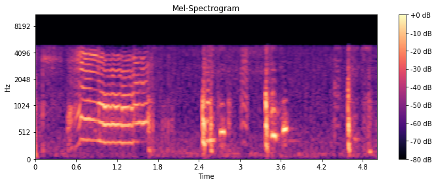
\includegraphics[width=1.2\linewidth]{first.png}
    \label{fig:mpr}
\end{figure}


\noindent Almost every major company in the field of IT technology has its own text-to-speech service. They are most often used in translation programs, as voice assistants in search engines and companies providing 
services, such as banks. Here is a comparative table of some of these services.
\newline
\newline

\begin{tabular}{ r|c|c| }
	\multicolumn{1}{r}{} &  \multicolumn{1}{c}{Google cloud text-to-speech } & \multicolumn{1}{c}{Amazon’s Polly}\\
	Real-time audio transmission & + & + \\
	\cline{2-3} SSML & + & +\\
	\cline{2-3} Custom Voice & + & - \\

\end{tabular} \\ 
\newpage



\section{Stages of processing}
\subsection{Normalization}

The main task of normalization is to bring the text to a standard unified form. This is necessary for further processing steps so that the acoustic model can unambiguously interpret and transform the text. Thus, we bring our text closer to the form in which it is used in oral speech. Usually, abbreviations, special symbols and numbers are subject to normalization.
\newline

\paragraph{Examples of text that need to be normalized:}

\begin{itemize}[noitemsep]
	\item $1917 \rightarrow$ nineteen seventeen
	\item kg $\rightarrow$ kilogram
	\item 10:00 $\rightarrow$ ten o’clock \ldots 
\end{itemize}

\begin{center}
    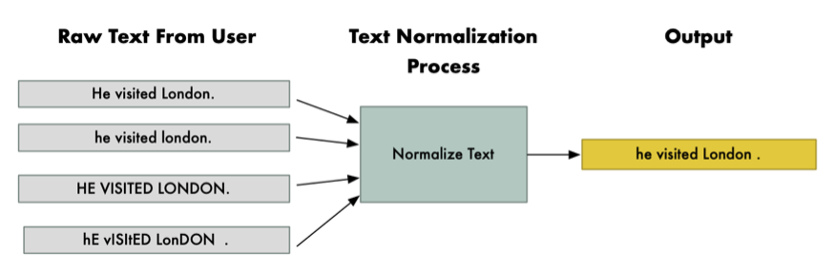
\includegraphics[width=0.6\linewidth]{second.png}\quad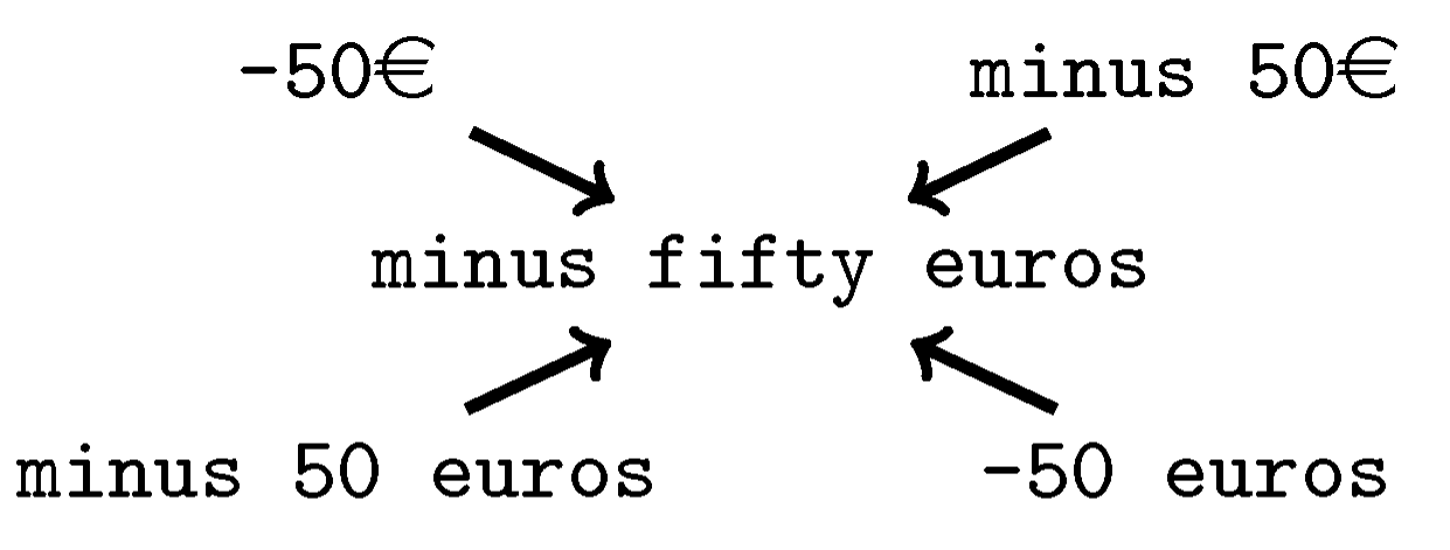
\includegraphics[width=0.3\linewidth]{third.png}
\end{center}

\noindent Finite State Transducer is a graph that has an initial and final state. The transducer takes input data, in our case, raw text, and produces output – normalized text. Each state of the transducer is connected by paths to a pair of input and output and, depending on the input, moves between states. Thus, WFST has a weighted sum on each edge, estimating the probability of issuing one or another result.  


\subsection{Acoustic}

The next step after NLP processing is the conversion of graphemes into mel-spectrograms. Such transformations from raw input text in our service are carried out by FastPitch, a fully feedforward Transformer model. The model consists of a bidirectional transducer, a pitch predictor, and a duration predictor. After passing through the first *N* blocks of the converter, encoding, the signal is supplemented with information about the pitch and discretely upsampled. It then goes through another set of *N* transformer blocks to smooth the upsampled signal and build a chalk spectrogram.
\newpage

\begin{figure}
\centering
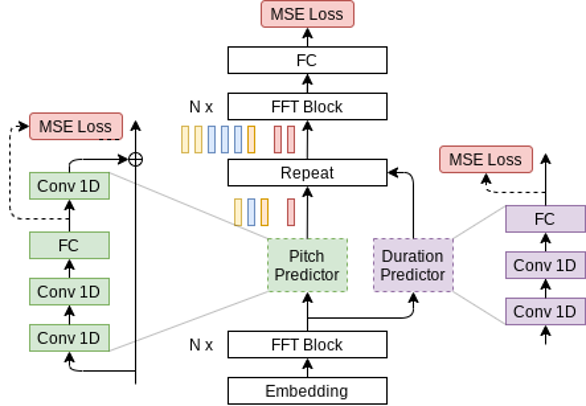
\includegraphics[width=1\linewidth]{fourth.png}
\caption{Acoustic model}
\end{figure}
\noindent The model is parallel, that allows you to quickly synthesize high-precision small-scale spectrograms with a high degree of control over speech parameters. The model provides the ability to adjust the tempo, expressiveness, pitch and intonation, which allows you to make the synthesized speech more natural.

\chapter{Bonus part}
This bonus part is about everything and nothing concrete))
\section{Genshin Impact}

This is my top 5 favourite characters is Genshin impact.
\begin{enumerate}  
	\item Xiao 
	\item Tartaglia 
	\item Zhongli
	\item Kaeya
	\item Kazuha
\end{enumerate}

\noindent This is list of items you shoud farm for you character to make him stringer.

\begin{enumerate}
	\item Weapon
	\item Artifacts
	\begin{enumerate}
		\item Flower
		\item Feather
		\item Watch
		\item Cup
		\item Crown
		\begin{enumerate}
		    \item Crit rate
		    \item Crit Damage
		\end{enumerate}
	\end{enumerate}
	\item Books for talents
	\item Items from bosses
\end{enumerate}

For dipper information you can check this \href{https://www.youtube.com/watch?v=U_ow8r_vuzs}{Xiao guide}
\newpage

\begin{center} 
Tier list of \textbf{main DD} \footnote{damage dealer} in Genshin.
\end{center}
\begin{tabular}{llll}
	\cellcolor{Red} S & Hu Tao 	& Ganyu & Ayaka\\
	\cellcolor{Gray} A 	& Xiao 	& Diluc & Yanfei\\
	\cellcolor{Green} B	& Kequing 	& Kaeya & Noelle \\
\end{tabular}
\section{Some math}

\begin{equation}
        \small{sin(\alpha + \beta) = sin\alpha cos\beta + cos\alpha sin\beta}
    \end{equation}

\begin{equation}
        \frac{n!}{k!(n-k)!} = \binom{n}{k}
    \end{equation}
    
\begin{equation}
  x = a_0 + \cfrac{1}{a_1 
          + \cfrac{1}{a_2 
          + \cfrac{1}{a_3 + \cfrac{1}{a_4} } } }
\end{equation}
\begin{equation}
    p_n(x) = p_{n-1}(x) + \frac{f^{(n)}(x_0)}{n!}(x-x_0)^n
\end{equation}\\

\begin{displayquote}
     \textsl{"Mathematics is the key and the door to all sciences." ©  Galileo Galilei}
\end{displayquote}
\begin{thebibliography}{}
\bibitem{}Eric Engelhart, Mahsa Elyasi, Gaurav Bharaj "Grapheme-to-Phoneme Transformer Model for Transfer Learning Dialects" \\
\bibitem{}Jungil Kong, Jaehyeon Kim, Jaekyoung Bae "HiFi-GAN: Generative Adversarial Networks for Efficient and High Fidelity Speech Synthesis" \\
\bibitem{}Evelina Bakhturina, Yang Zhang, Boris Ginsburg "Shallow Fusion of Weighted Finite-State Transducer and Language Model for Text Normalization" \\
\end{thebibliography}
\end{document}
